\documentclass[addpoints]{exam}

\usepackage{caption}
\usepackage{graphbox}
\usepackage{hyperref}
\usepackage{listings}
\usepackage{multirow}
\usepackage{ragged2e}
\usepackage{subcaption}
\usepackage{tabularx}
\usepackage{xcolor}

% Header and footer.
\pagestyle{headandfoot}
\runningheadrule
\runningfootrule
\runningheader{CS 201 Data Structures II}{HW 2: Skiplists and Hash Tables}{Spring 2021}
\runningfooter{}{Page \thepage\ of \numpages}{}
\firstpageheader{}{}{}

\qformat{{\large\bf \thequestion. \thequestiontitle}\hfill[\totalpoints\ points]}
% \qformat{{\large\bf \thequestion. \thequestiontitle}\hfill}
\boxedpoints

\printanswers

\graphicspath{{images/}}

\newcommand\colheader[1]{\multicolumn{1}{c}{#1}} % Note: no vertical bars

% Colored Python listing from https://www.overleaf.com/learn/latex/Code_listing
\definecolor{codegreen}{rgb}{0,0.6,0}
\definecolor{codegray}{rgb}{0.5,0.5,0.5}
\definecolor{codepurple}{rgb}{0.58,0,0.82}
\definecolor{backcolour}{rgb}{0.95,0.95,0.92}
 
\lstdefinestyle{mystyle}{
    backgroundcolor=\color{backcolour},   
    commentstyle=\color{codegreen},
    keywordstyle=\color{magenta},
    numberstyle=\tiny\color{codegray},
    stringstyle=\color{codepurple},
    basicstyle=\ttfamily\footnotesize,
    breakatwhitespace=false,         
    breaklines=true,                 
    captionpos=b,                    
    keepspaces=true,                 
    numbers=left,                    
    numbersep=5pt,                  
    showspaces=false,                
    showstringspaces=false,
    showtabs=false,                  
    tabsize=2
}
\lstset{style=mystyle}

\title{Homework 2: Skiplists and Hash Tables}
\author{CS 201 Data Structures II\\Habib University\\Spring 2021}
\date{}  % <=== Enter your team name.

\begin{document}
\maketitle
\part{Skiplists}

The solutions to the following problems are to be entered inline below. Remove all other parts and sections from this document. Enter your team name for the date in the document's title.

\begin{questions}

\titledquestion{Redundant Comparisons}\footnote{Adapted from Exercise 4.8 in the textbook.}
  The \texttt{find(x)} method in a \texttt{SkiplistSet} sometimes performs redundant comparisons; these occur when \texttt{x} is compared to the same value more than once. They can occur when, for some node, \texttt{u}, \texttt{u.next[r] = u.next[r-1]}.
  \begin{parts}
  \part[5] What causes these redundant comparisons to happen?
    \begin{solution}
      % Enter your solution here.
    \end{solution}
  \part[5] Modify \texttt{find(x)} so that redundant comparisons are avoided.
    \begin{solution}
      % Enter your solution here.
    \end{solution}
  \end{parts}

\titledquestion{A Ranked Set}[10]\footnote{Adapted from Exercise 4.9 in the textbook.}
  Design, a version of a skiplist that implements the \texttt{SSet} interface, but also allows fast access to elements by \textit{rank}. That is, it also supports the function \texttt{get(i)}, which returns the element whose rank is \texttt{i} in $O(\log n)$ expected time. (The rank of an element \texttt{x} in an \texttt{SSet} is the number of elements in the \texttt{SSet} that are less than \texttt{x}.)

  Describe how your version differs from a regular skiplist and provide pseudocode of \texttt{find(x)} and \texttt{get(i)} for this version.
  \begin{solution}
    % Enter your solution here.
  \end{solution}

\titledquestion{Finger Search}[10]\footnote{Adapted from Exercise 4.10 in the textbook.}
  A \textit{finger} in a skiplist is an array that stores the sequence of nodes on a search path at which the search path goes down. (The variable \texttt{stack} in the \texttt{add(x)} code on page 87 is a finger; the shaded nodes in Figure 4.3 show the contents of the finger.) One can think of a finger as pointing out the path to a node in the lowest list, $L_0$.
  
  A \textit{finger search} implements the find(x) operation using a finger, walking up the list using the finger until reaching a node \texttt{u} such that \texttt{u.x < x} and \texttt{u.next = nil} or \texttt{u.next.x > x} and then performing a normal search for \texttt{x} starting from \texttt{u}. It is possible to prove that the expected number of steps required for a finger search is $O(1+\log r)$, where $r$ is the number values in $L_0$ between \texttt{x} and the value pointed to by the finger.

  Design, i.e. provide the necessary pseudo code for, a version of a skiplist that implements \texttt{find(x)} operations using an internal finger. This subclass stores a finger, which is then used so that every \texttt{find(x)} operation is implemented as a finger search. During each \texttt{find(x)} operation the finger is updated so that each \texttt{find(x)} operation uses, as a starting point, a finger that points to the result of the previous \texttt{find(x)} operation.
  \begin{solution}
    % Enter your solution here.
  \end{solution}
\end{questions}

\part{Hash Tables}

\begin{figure}[!h]
  \centering
  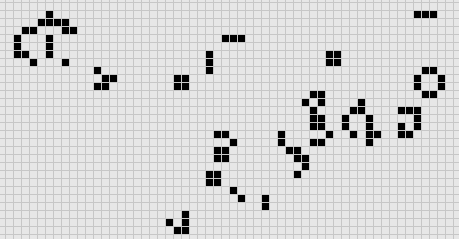
\includegraphics[scale=.8]{banner}
  \caption{A sample game state in Conway's Game of Life. From \href{http://pi.math.cornell.edu/~lipa/mec/lesson6.html}{Chaos and Fractals: Conway's Game of Life}.}
\end{figure}

In this assignment, we will implement 2 different hash tables which differ in their conflict resolution strategy. We will use the hash table to implement Conway's Game of Life.

\section{Game of Life}
\label{sec:imgops}

\begin{quotation}
\href{https://en.wikipedia.org/wiki/Conway's_Game_of_Life}{Conway’s Game of Life} is a simple simulation with surprisingly complex behavior. We start with a simple 2D grid of cells. Each cell can be either alive or dead. The rules are:
\begin{itemize}
\item A live cell stays alive if it has two or three live neighbors.
\item A dead cell becomes alive if it has exactly three live neighbors.
\end{itemize}
We start with a certain set of cell states and then iterate, applying the rules to every cell at each iteration. Despite their simplicity, these rules can produce amazingly complicated behavior.
\end{quotation}
\raggedleft --- \href{https://www.refsmmat.com/posts/2016-01-25-conway-game-of-life.html}{A flexible implementation of Conway's Game of Life}
\justify
The rules above are presented differently from their original formulation but they are nonetheless correct. This formulation is presented because it is more amenable to our eventual implementation.

\subsection{Initial Configurations}

The game begins with an initial configuration of live cells. This constitutes the starting state of the game. As the rules of the game are deterministic, the starting state completely determines all subsequent states of the game. Some initial configurations lead to interesting behavior and have led to the identification of certain classes of patterns.
\begin{description}
\item[Still Life] These patterns are not affected by further iterations of the game and stay unchanged as the game proceeds.
\item[Oscillators] These patterns recur after a fixed number of iterations which are called the \textit{period} of the oscillator.
\item[Spaceships] These are oscillators that change position or \textit{glide} across the grid.
\end{description}

\begin{figure}[!h]
  \centering
  \begin{tabular}{cc}
    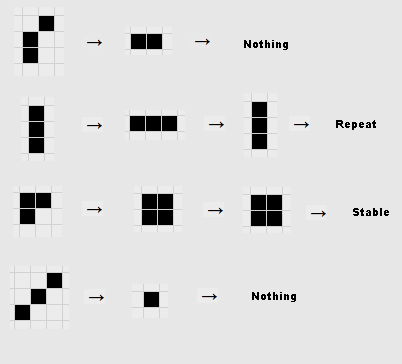
\includegraphics[width=.48\textwidth]{pattern1}
    & 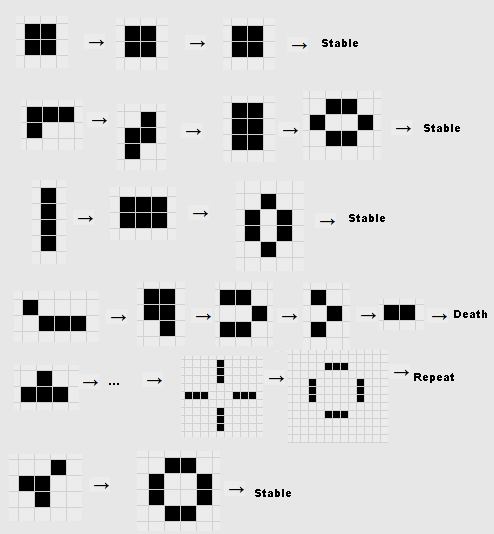
\includegraphics[width=.48\textwidth]{pattern2}
  \end{tabular}
  \caption{Evolution of the game from some initial states. From \href{http://pi.math.cornell.edu/~lipa/mec/lesson6.html}{Chaos and Fractals: Conway's Game of Life}.}
\end{figure}


\subsection{Computation}
\begin{quotation}
  It's possible even, to create patterns which emulate logic gates (and, not, or, etc.) and counters. Building up from these, it was proved that the Game of Life is \href{https://simple.wikipedia.org/wiki/Turing_complete}{Turing Complete}, which means that with a suitable initial pattern, one can do any computation that can be done on any computer. Later, Paul Rendell actually constructed a simple Turing Machine as a proof of concept, which can be found \href{https://www.ics.uci.edu/~welling/teaching/271fall09/Turing-Machine-Life.pdf}{here}.
\end{quotation}
\raggedleft --- \href{http://pi.math.cornell.edu/~lipa/mec/lesson6.html}{Chaos and Fractals: Conway's Game of Life}
\justify
Some links in the above excerpt that are now dead have been updated.

\subsection{Visualization}

As the Game of Life is a dynamic system, i.e. its state changes with each iteration, it is best viewed as an animation which this document is unable to present. See the \href{https://en.wikipedia.org/wiki/Conway's_Game_of_Life}{Wikipedia page} or any of the other pages linked in this document for helpful animations. Here is a \href{https://www.youtube.com/watch?v=C2vgICfQawE}{YouTube video}.

\section{Implementation Details}

An implementation of Conway's Game of Life is provided in the accompanying file \texttt{game.py} whose contents are also presented in the Appendix in this document. The file contains two main classes.

\paragraph{\texttt{Life}} Every instance is initialized with a starting configuration which is stored using two different hash tables.\\
--- \texttt{self.\_alive} stores the two-dimensional $(x,y)$ coordinates of \texttt{live cells}\\\smallskip
--- \texttt{self.\_nbr\_count} stores \textit{neighbor information} as key-value pairs where each key is an $(x,y)$ coordinate of a cell with \textit{live neighbors} and its value is the number of its live neighbors.\\
The hash tables store not only the initial configuration but, once the game starts, they store the state of the game at the end of each iteration. During each iteration, the live cells have to be used to populate neighbor information which in turn must be used to update the live cells. This is already coded in the \texttt{step} method of \texttt{Life}. \textit{Do not modify} the implementation of this class.

\paragraph{\texttt{Game}} It runs a \texttt{Life} instance according to the provided configurations with an option for animation. In the animation system used, the origin, $(0,0)$, is at the top left of the window. This class is provided for your testing. \textit{You may modify} it as per your needs.

\section{Task}

Your task is to implement the two hash tables in \texttt{Life} using two different conflict resolution methods. Specifically, you have to implement the following classes which are utilized in the implementation of \texttt{Life}.
\begin{description}
\item[\texttt{ChainedSet}] A hash table that implements the \texttt{USet} interface using chaining for conflict resolution.
\item[\texttt{ChainedDict}] A hash table that implements the \texttt{USet} interface as an associative container and uses chaining for conflict resolution.
\item[\texttt{LinearSet}] A hash table that implements the \texttt{USet} interface using linear probing for conflict resolution.
\item[\texttt{LinearDict}] A hash table that implements the \texttt{USet} interface as an associative container and uses linear probing for conflict resolution.
\end{description}
The conflict resolution strategy to use is indicated through a parameter passed to \texttt{Life} at the time of initialization.

Make sure to go over the provided implementation first in order gain a good understanding of the game logic and the requirements, specifically the interface that the hash tables must support.
  
\section*{Credits}

The Game of Life homework is adapted from \href{https://www.refsmmat.com/posts/2016-01-25-conway-game-of-life.html}{A flexible implementation of Conway's Game of Life}.

\newpage

\appendix
\part*{Appendix}
The listings below are based on real time retrieval of line numbers from the accompanying file, \texttt{game.py}. Modifying the file will change the listings.

\section{The \texttt{Life} class}
\lstinputlisting[language=python, frame=single, linerange={51-123}]{game.py}

\section{The \texttt{Game} class}
\lstinputlisting[language=python, frame=single, linerange={126-169}]{game.py}

\end{document}
%%% Local Variables:
%%% mode: latex
%%% TeX-master: t
%%% End:
